\documentclass[11pt]{opticajnl}
\journal{opticajournal} % use for journal or Optica Open submissions

% See template introduction for guidance on setting shortarticle option
\setboolean{shortarticle}{true}
% true = letter/tutorial
% false = research/review article

% ONLY applicable for journal submission shortarticle types:
% When \setboolean{shortarticle}{true}
% then \setboolean{memo}{true} will print "Memorandum" on title page header
% Otherwise header will remain as "Letter"
% \setboolean{memo}{true}
\usepackage{lineno}
\usepackage{listings}
\usepackage{xcolor}  % Para colorear el código

% Definir colores para la sintaxis de Python
\definecolor{pystring}{RGB}{186,33,33}      % Strings
\definecolor{pycomment}{RGB}{107,107,107}   % Comentarios
\definecolor{pykeyword}{RGB}{0,119,170}     % Palabras clave
\definecolor{pybuiltin}{RGB}{163,21,21}     % Funciones builtin
\definecolor{pybackground}{RGB}{250,250,250} % Fondo

% Definir el estilo para código Python
\lstdefinestyle{Python}{
    language=Python,
    backgroundcolor=\color{pybackground},
    basicstyle=\ttfamily\small,
    breakatwhitespace=false,
    breaklines=true,
    captionpos=b,
    keepspaces=true,
    numbers=left,
    numbersep=5pt,
    showspaces=false,
    showstringspaces=false,
    showtabs=false,
    tabsize=4,
    frame=single,
    commentstyle=\color{pycomment},
    keywordstyle=\color{pykeyword},
    stringstyle=\color{pystring},
    identifierstyle=\color{black},
    numberstyle=\tiny\color{gray},
    emphstyle=\color{pybuiltin},
    morekeywords={import,from,as,def,class,return,yield,for,while,if,else,elif,
                  try,except,finally,with,lambda,assert,pass,break,continue,
                  raise,global,nonlocal,True,False,None,and,or,not,is,in},
    emph={pandas,numpy,matplotlib,seaborn,sklearn,tensorflow,torch,
          plt,pd,np,sns,print,len,range,enumerate,zip,dict,list,tuple,set,
          min,max,sum,sorted,map,filter},
}

\lstdefinestyle{sql}{
  language=SQL,
  showspaces=false, 
  basicstyle=\ttfamily,
  numbers=left,
  numberstyle=\tiny,
  backgroundcolor=\color{gray!10},
  keywordstyle=\color{blue}\bfseries,
  commentstyle=\color{green!70}\ttfamily,
  stringstyle=\color{red!70}\ttfamily,
  breaklines=true,
  morekeywords={CREATE, DROP, TABLE, SELECT, INSERT, UPDATE, DELETE, FROM, WHERE, JOIN, ON, AS}, % Puedes añadir más palabras clave específicas de SQL.
  literate={``}{``}1 {''}{''}1 {“}{``}1 {”}{''}1 {‘}{`}1 {’}{'}1
}

\lstdefinestyle{terminal}{
  backgroundcolor=\color{white},   % Fondo blanco
  basicstyle=\color{black}\ttfamily, % Texto negro en fuente monoespaciada
  keywordstyle=\color{blue}\bfseries, % Palabras clave en azul y negrita
  commentstyle=\color{green!70}\ttfamily, % Comentarios en verde
  stringstyle=\color{red}\ttfamily, % Cadenas en rojo
  morekeywords={sudo, apt-get, install, cd, ls, mkdir, rm, rmdir, cp, mv, echo, cat, nano, vim, grep, find, chmod, chown, systemctl, service, update, upgrade, reboot, shutdown, exit}, % Comandos comunes de terminal
  breaklines=true, % Permitir saltos de línea
  frame=single, % Marco alrededor del código
  framerule=0.5pt, % Grosor del marco
  rulecolor=\color{gray}, % Color del marco
  xleftmargin=0.05\textwidth, % Margen izquierdo
  xrightmargin=0.05\textwidth, % Margen derecho
  aboveskip=1em, % Espacio antes del bloque de código
  belowskip=1em % Espacio después del bloque de código
}
\definecolor{rstring}{RGB}{186,33,33}     % Strings
\definecolor{rcomment}{RGB}{0,128,0}      % Comentarios
\definecolor{rfunction}{RGB}{0,0,255}      % Funciones
\definecolor{rkeyword}{RGB}{145,0,145}    % Palabras clave
\definecolor{rbackground}{RGB}{248,248,248} % Fondo

\lstdefinestyle{R}{
    language=R,
    backgroundcolor=\color{rbackground},
    basicstyle=\ttfamily\small,
    breakatwhitespace=false,
    breaklines=true,
    captionpos=b,
    keepspaces=true,
    numbers=left,
    numbersep=5pt,
    showspaces=false,
    showstringspaces=false,
    showtabs=false,
    tabsize=2,
    frame=single,
    commentstyle=\color{rcomment},
    keywordstyle=\color{rkeyword},
    stringstyle=\color{rstring},
    identifierstyle=\color{black},
    numberstyle=\tiny\color{gray},
    morekeywords={library, data.frame, read.csv, ggplot, aes, geom_bar, theme_minimal, 
                  scale_fill_manual, gather, group_by, summarise, arrange, filter},
}


%\linenumbers % Turn off line numbering for Optica Open preprint submissions.

\title{Dashboard con Tableau}

\author[1,2,3]{Luis Ardévol Mesa}


\begin{abstract}
El objetivo de esta práctica es crear un dashboard permita avanzar en conocimiento sobre aspectos relacionados con el tráfico aéreo global. En este caso, se hará un análisis de la conectividad entre los distintos países, lo que permite ver las tendencias del tráfico aéreo internacional, identificar \textit{hubs}, etc.
\end{abstract}

\setboolean{displaycopyright}{false} % Do not include copyright or licensing information in submission.

\begin{document}

\maketitle

No se entrará en detalles acerca de la carga de los datos en Tableau; esta simplemente se realiza mediante la importación de la base de datos de PostgreSQL existente en nuestra máquina virtual, \textit{backup\_vuelos}, haciendo uso del puerto 5432. \\

Con este \textit{dashboard} se pretende comprender, de la forma más sencilla posible, un sistema tan complejo como es el tráfico aéreo en la actualidad. Países como Estados Unidos o China, presentan un gran número de rutas, tanto nacionales como internacionales. Otros países como España y Alemania presentan un mayor número de rutas internacionales que nacionales, mientras que, con otros países, se tiene el caso contrario. Existen también países con vuelos exclusivamente internacionales: esto ocurre con las islas, que generalmente tienen un único aeropuerto (o dos, pero la conexión entre ellos es infrecuente). \\

Este análisis de conectividad se puede usar para comprender mejor las rutas ya existentes, posibles mejoras en ellas, eliminación de las mismas o incluso creación de nuevas rutas. Además, permite ver las tendencias en el tráfico aéreo global, identificando \textit{hubs} o aeropuertos que reunen una parte considerable del tráfico. \\

Esto se hará mediante tres visualizaciones: la primera mostrará las rutas aéreas existentes. Al ser un número elevado, se acompañará de un filtro que permite seleccionar el país (o países) a mostrar, lo que permite un análisis en profundidad de cada país. La segunda visualización será un mapa de calor de los países con mayor número de rutas y la tercera, siguiendo la línea de la segunda, será una matriz (o tabla) de calor, que muestre el número de rutas entre distintos países. Estas dos últimas van de la mano, por lo que usarán la misma escala y compartirán filtros para una mejor comprensión del problema que se quiera abordar. \\

Para realizar estas visualizaciones basta con conectar la tabla de rutas con la tabla de aeropuertos. Esto se debe hacer dos veces: una para el aeropuerto de origen, conectando \textit{source\_airport\_id}, de la tabla \textit{routes} con \textit{airport\_id}, de la tabla \textit{airports}, y otra para el aeropuerto de destino, conectando \textit{destination\_airport\_id}, de la tabla \textit{routes} con \textit{airport\_id}, de la tabla \textit{airports}. Se adjuntará el código de cualquier campo cálculado creado para las visualizaciones. Cualquier campo del que no se haga mención de su creación, ya venía en la propia base de datos. 

\section{Mapa de rutas}

Para realizar el mapa de rutas, primero se deben crear tres campos calculados:
\begin{itemize}
\item Uno para el punto de origen: \textit{Origin point}
\begin{lstlisting}[style=terminal]
MAKEPOINT([Latitude], [Longitude])
\end{lstlisting}
\item Uno para el punto de destino: \textit{Destination point}
\begin{lstlisting}[style=terminal]
MAKEPOINT([Latitude (Airports1)], [Longitude (Airports1)])
\end{lstlisting}
\item Uno para la ruta que conecta los puntos de origen y destino: \textit{Flight Path}
\begin{lstlisting}[style=terminal]
MAKELINE([Origin point], [Destination point])
\end{lstlisting}
\end{itemize}

con estos campos se definen los aeropuertos de origen y destino como puntos, y se crea una línea que los une. Para mostrarlo sobre el mapa, se añade el campo \textit{Longitud (generado)} como columnas y el campo \textit{Latitud (generado)} como filas. Esto genera un mapa vacío en la hoja actual. El estilo del mapa se puede modificar haciendo \textit{click} derecho sobre le mismo y entrando en ``capas en segundo plano''; en este caso, se selecciona el estilo ``normal''. Añadiendo \textit{Flight Path} a los detalles de la visualización, ya se tiene lo básico. \\

Para discriminar rutas a simple vista, se elige que el color de las mismas varíe con la distancia de las mismas. Esto se consigue agregando el campo \textit{Distancia Km} el apartado de color, usando el promedio como función de agregado. Además, resulta conveniente reducir el tamaño o grosor de las líneas, para evitar \textit{overploting} (aunque dependiente del país seleccionado, esto resulta imposible). \\

Para hacer un análisis, resulta interesante conocer datos acerca de cada ruta. En este caso, se mostrarán los aeropuertos de origen y destino (acompañados de sus respectivos países), el número de rutas entre ellos y la distancia promedio en kilómetros. Así, la descripción emergente usada tiene esta forma: 
\begin{lstlisting}[style=terminal]
Origen:	<Name> (<Pais Origen>)
Destino: <Name (Airports1)> (<Pais Destino>)
Rutas: <REC(routes)>
Distancia Km: <PROM(Distancia Km)>
\end{lstlisting}

\begin{figure}[h]
\centering
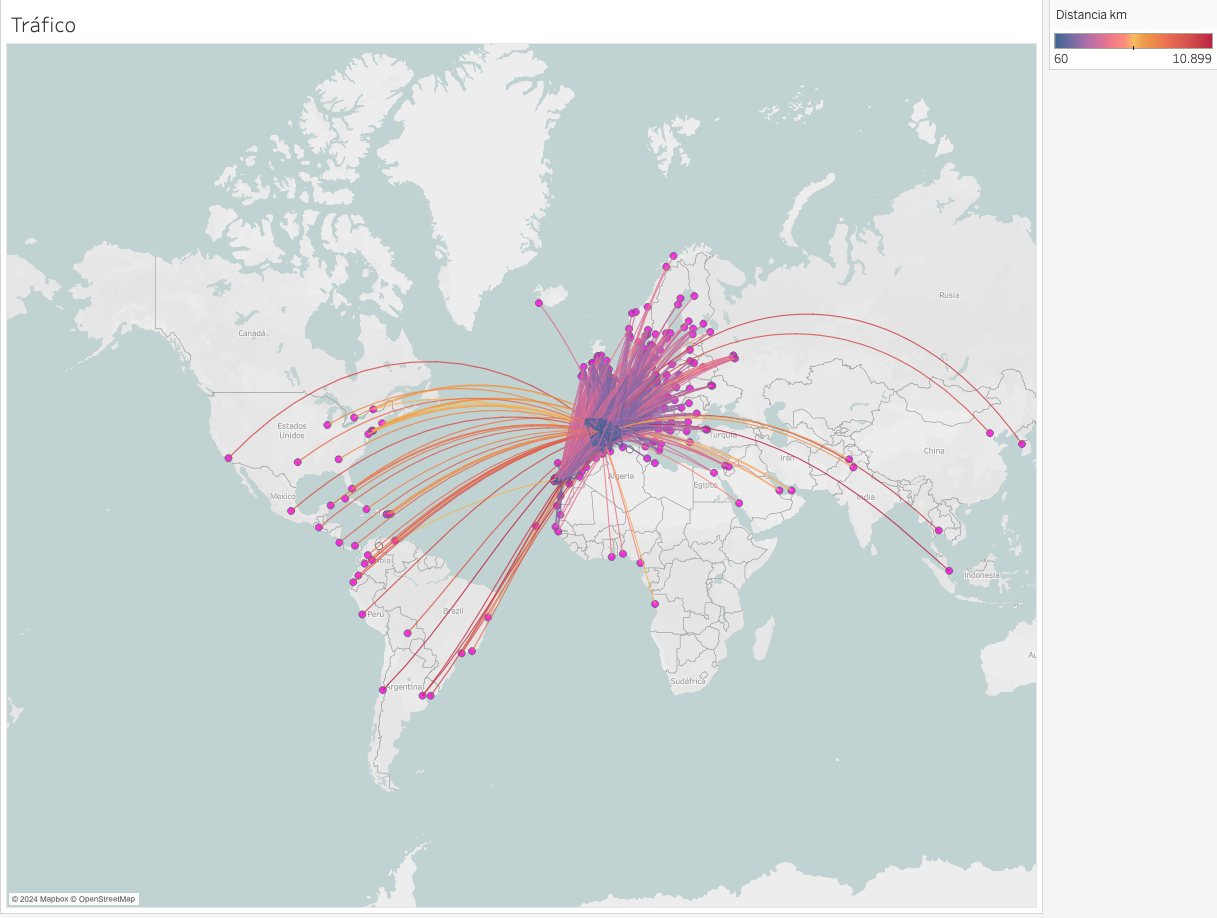
\includegraphics[width=0.62\textwidth]{fotos/1.png}
\caption{Mapa de rutas, filtrando como país de origen España.}
\label{fig:1}
\end{figure}

Para dar mayor completitud, los aeropuertos, tanto de origen (color blanco) como de destino (color rosa), se muestran con puntos lo más pequeños posible. Esto se consigue creando una nueva capa para cada uno: arrastrando el campo \textit{Origin point} sobre el mapa, se agrega a una nueva capa, donde solo se agregará como información el nombre del aeropuerto correspondiente a cada punto. Del mismo, se crea una capa nueva con el campo \textit{Destination point}. \\

Esta visualización irá acompañada de una leyenda de color acerca de la distancia en kilómetros. Los filtros se agregarán posteriormente en el propio \textit{dashboard}, aunque para mostrarlo en la figura \ref{fig:1}, se selecciona un único país, España. 

\section{Mapa de calor}

Esta visualización consiste de nuevo en un mapa que, esta vez, muestre el número de rutas con origen en cada país. Para ello, una opción sencilla de interpretar es un mapa de calor, donde cada país varíe su color en función del número de rutas. Lo primero es generar un mapa; esto se puede hacer de la misma forma que antes, con los campos \textit{Longitud (generado)} y \textit{Latitud (generado)}. \\

Se dispone de un campo que hace el recuento de rutas, \textit{routes (Recuento)}, por lo que se podría generar el mapa sin más que arrastrar este campo sobre el mismo. Sin embargo, analizando los datos, se puede apreciar un gran problema: hay países que rompen la escala por completo. Estados Unidos, con 13200 rutas, y China, con 8247 rutas, están muy lejos del resto de países, siendo los siguientes en la escala Reino Unido y España, con poco más de 2500 rutas. De hecho, el problema es aun mayor si nos damos cuenta de que, en realidad, son pocos los países que superan la barrera de las 500-600 rutas. Una escala lineal es por tanto una mala opción para esta representación, ya que no acentuaría la diferencia entre los países, sino entre los gigantes. 

\begin{figure}[h]
\centering
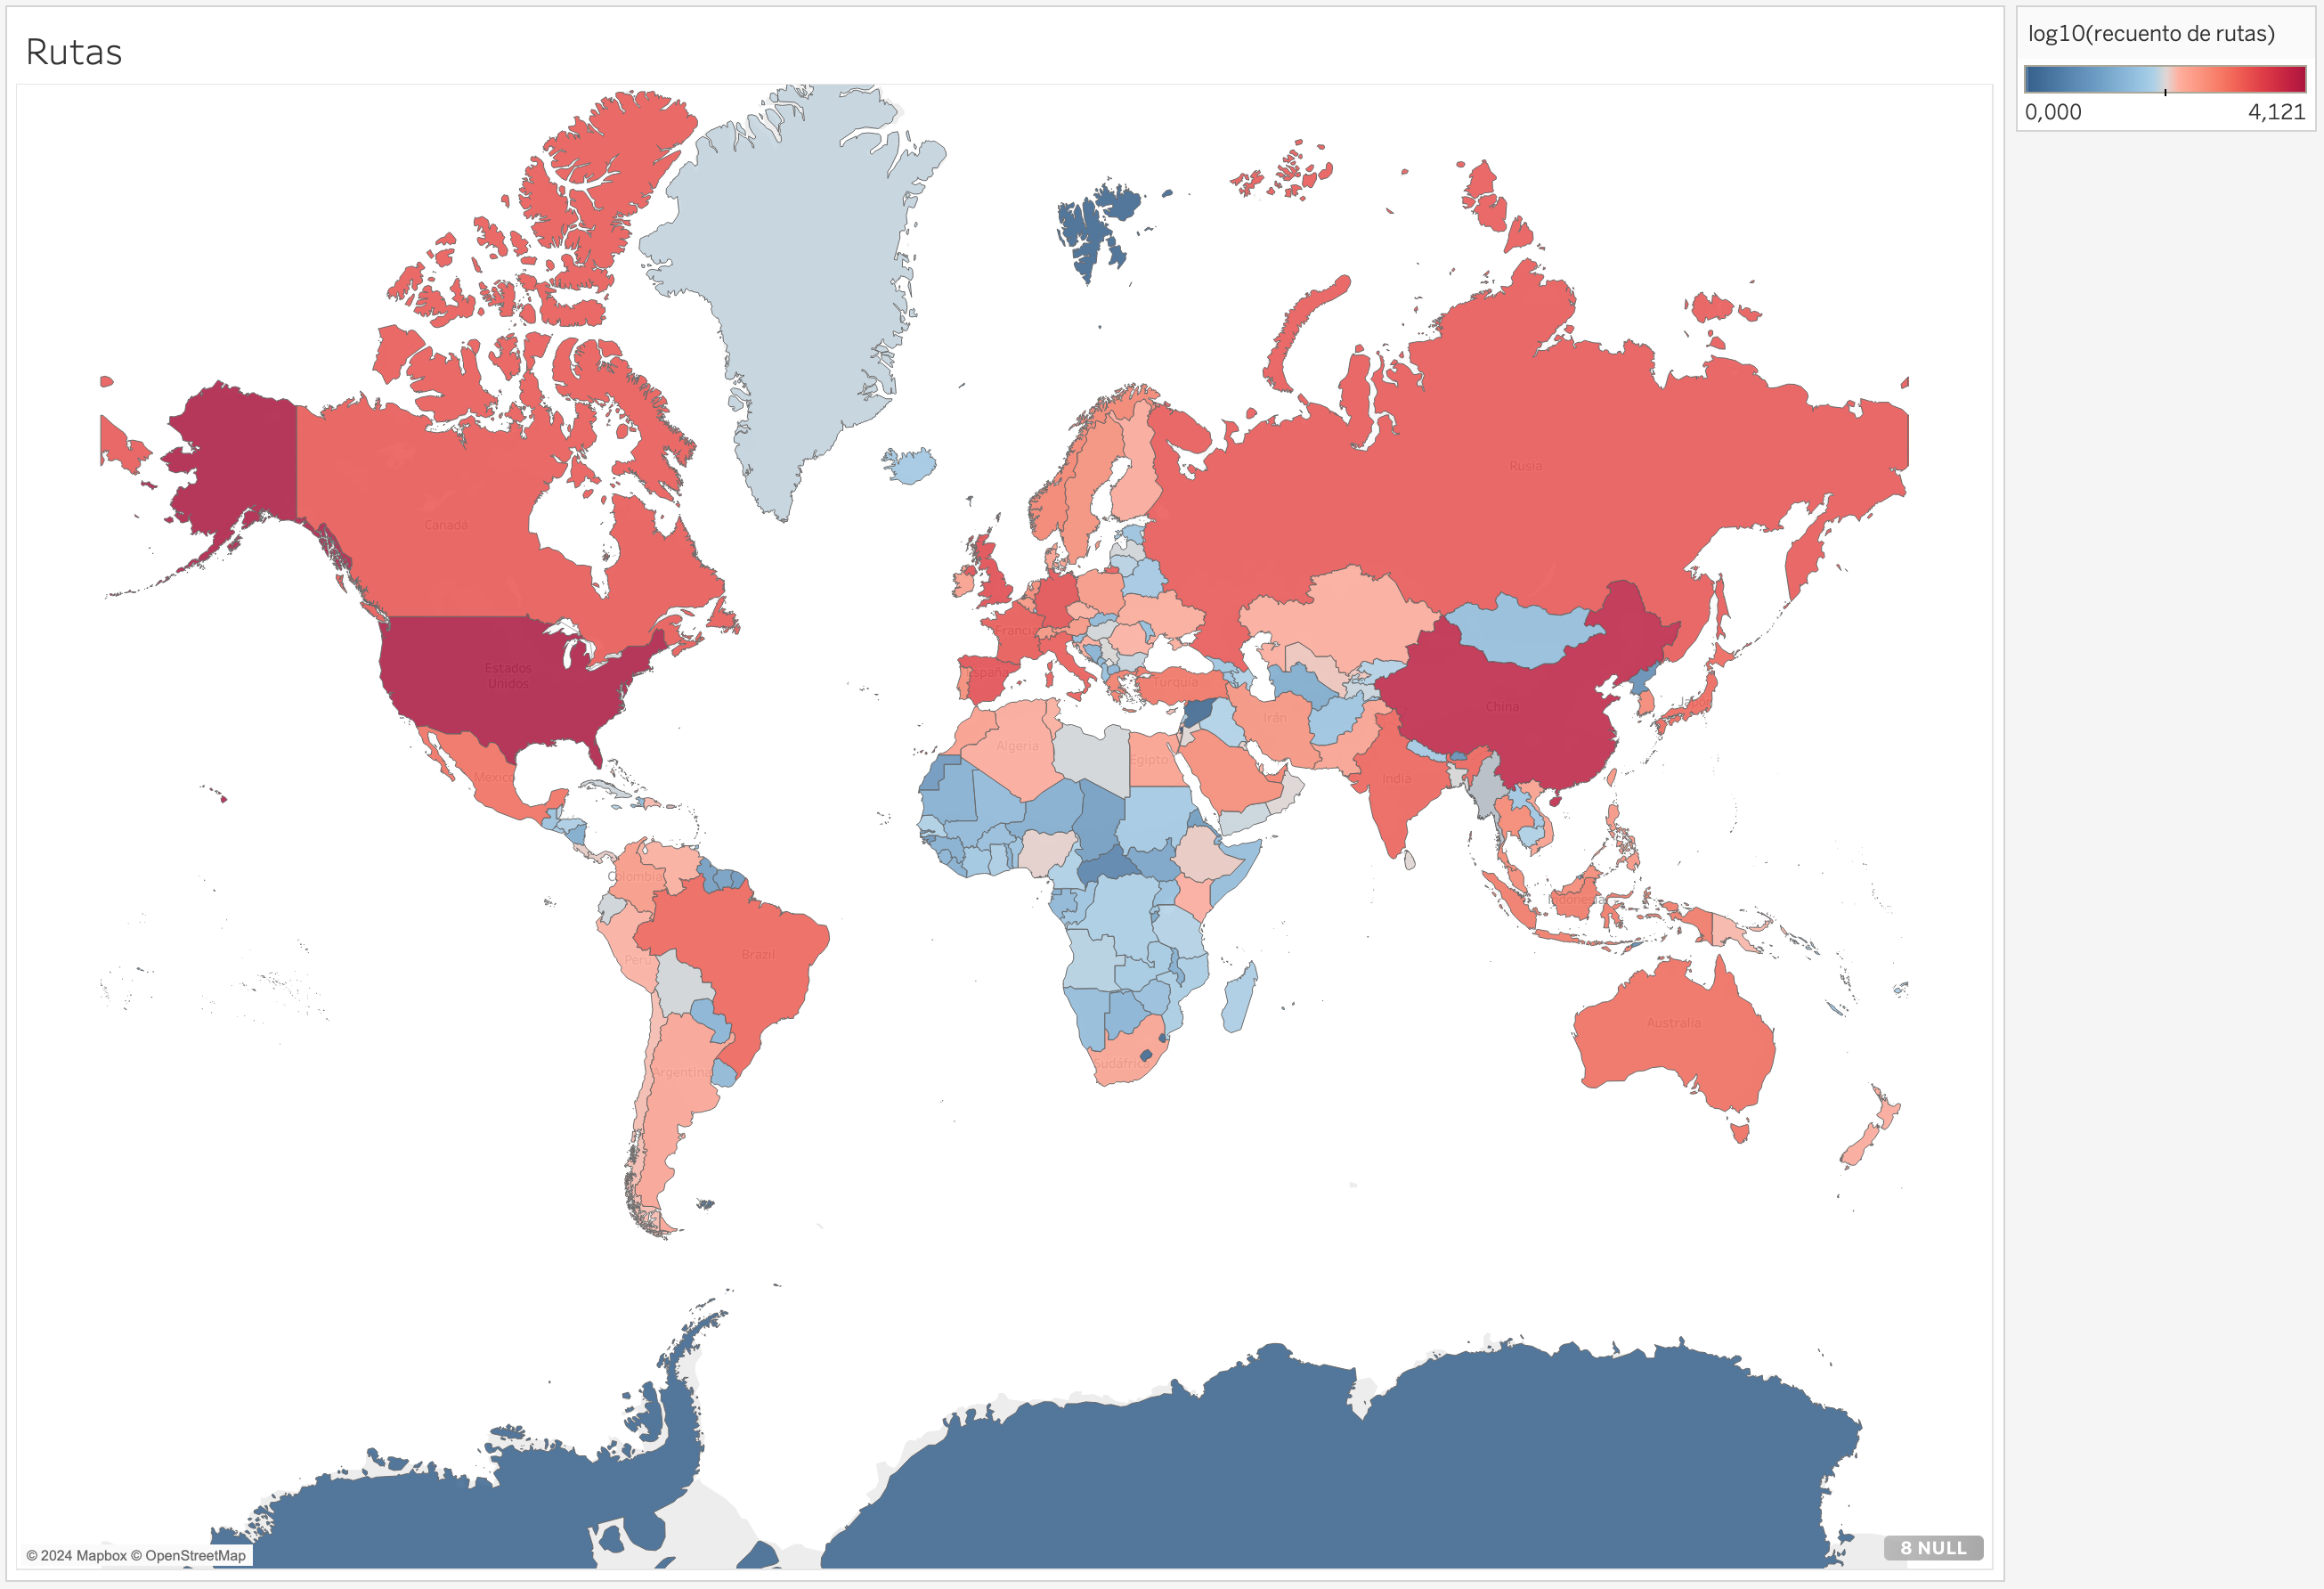
\includegraphics[width=0.7\textwidth]{fotos/2.png}
\caption{Mapa de calor del número de rutas por país.}
\label{fig:2}
\end{figure}

La solución al problema de la escala es simple: usar una escala logaritmica. Esto se consigue usando funciones numéricas de Tableau sobre el campo \textit{routes}. Se crea el campo calculado \textit{rutasLog} como 
\begin{lstlisting}[style=terminal]
LOG(COUNT([routes]))
\end{lstlisting}

Ahora arrastrando \textit{Pais Origen} (el nombre del país de origen, simplemente fue renombrado) sobre los detalles del mapa, y \textit{rutasLog} sobre el color, se obtiene el mapa de la figura \ref{fig:2}. \\

Se acompaña de nuevo de una leyenda con la correspondencia de los colores. Si bien la representación en escala logarítmica resulta intuitiva de forma visual (cuanto más oscuro sea el rojo, más rutas, y cuánto más oscuro el azul, menos rutas), no se puede saber de forma rápida a qué número de rutas corresponden esos colores a partir de la leyenda. Esto se arregla modificando la descripción emergente de cada país: 
\begin{lstlisting}[style=terminal]
Pais:	<Pais Origen>
Rutas:	<REC(routes)>
\end{lstlisting}

Con todo esto, resulta posible discernir las diferencias en la cantidad de ruta de cada país a simple vista, y para un análisis de mayor profundidad, es decir, conocer el número exacto, basta con situarnos sobre un país. En el \textit{dashboard} se añadirá un filtro de países para este mapa. 

\section{Matriz de calor}

La información proporcionada en el mapa anterior es buena, pero muy general. Estados Unidos y China tienen un gran número de rutas en comparación al resto de países, pero abarcan una gran superificie, por lo que pueden surgir preguntas: ¿cuántas de ellas son nacionales? ¿Y cuántas internacionales? ¿Con qué países tienen más rutas? Con el objetivo de conocer en mayor profundidad las conexiones de cada país, se hace esta matriz de calor. \\

\begin{figure}[h]
\centering
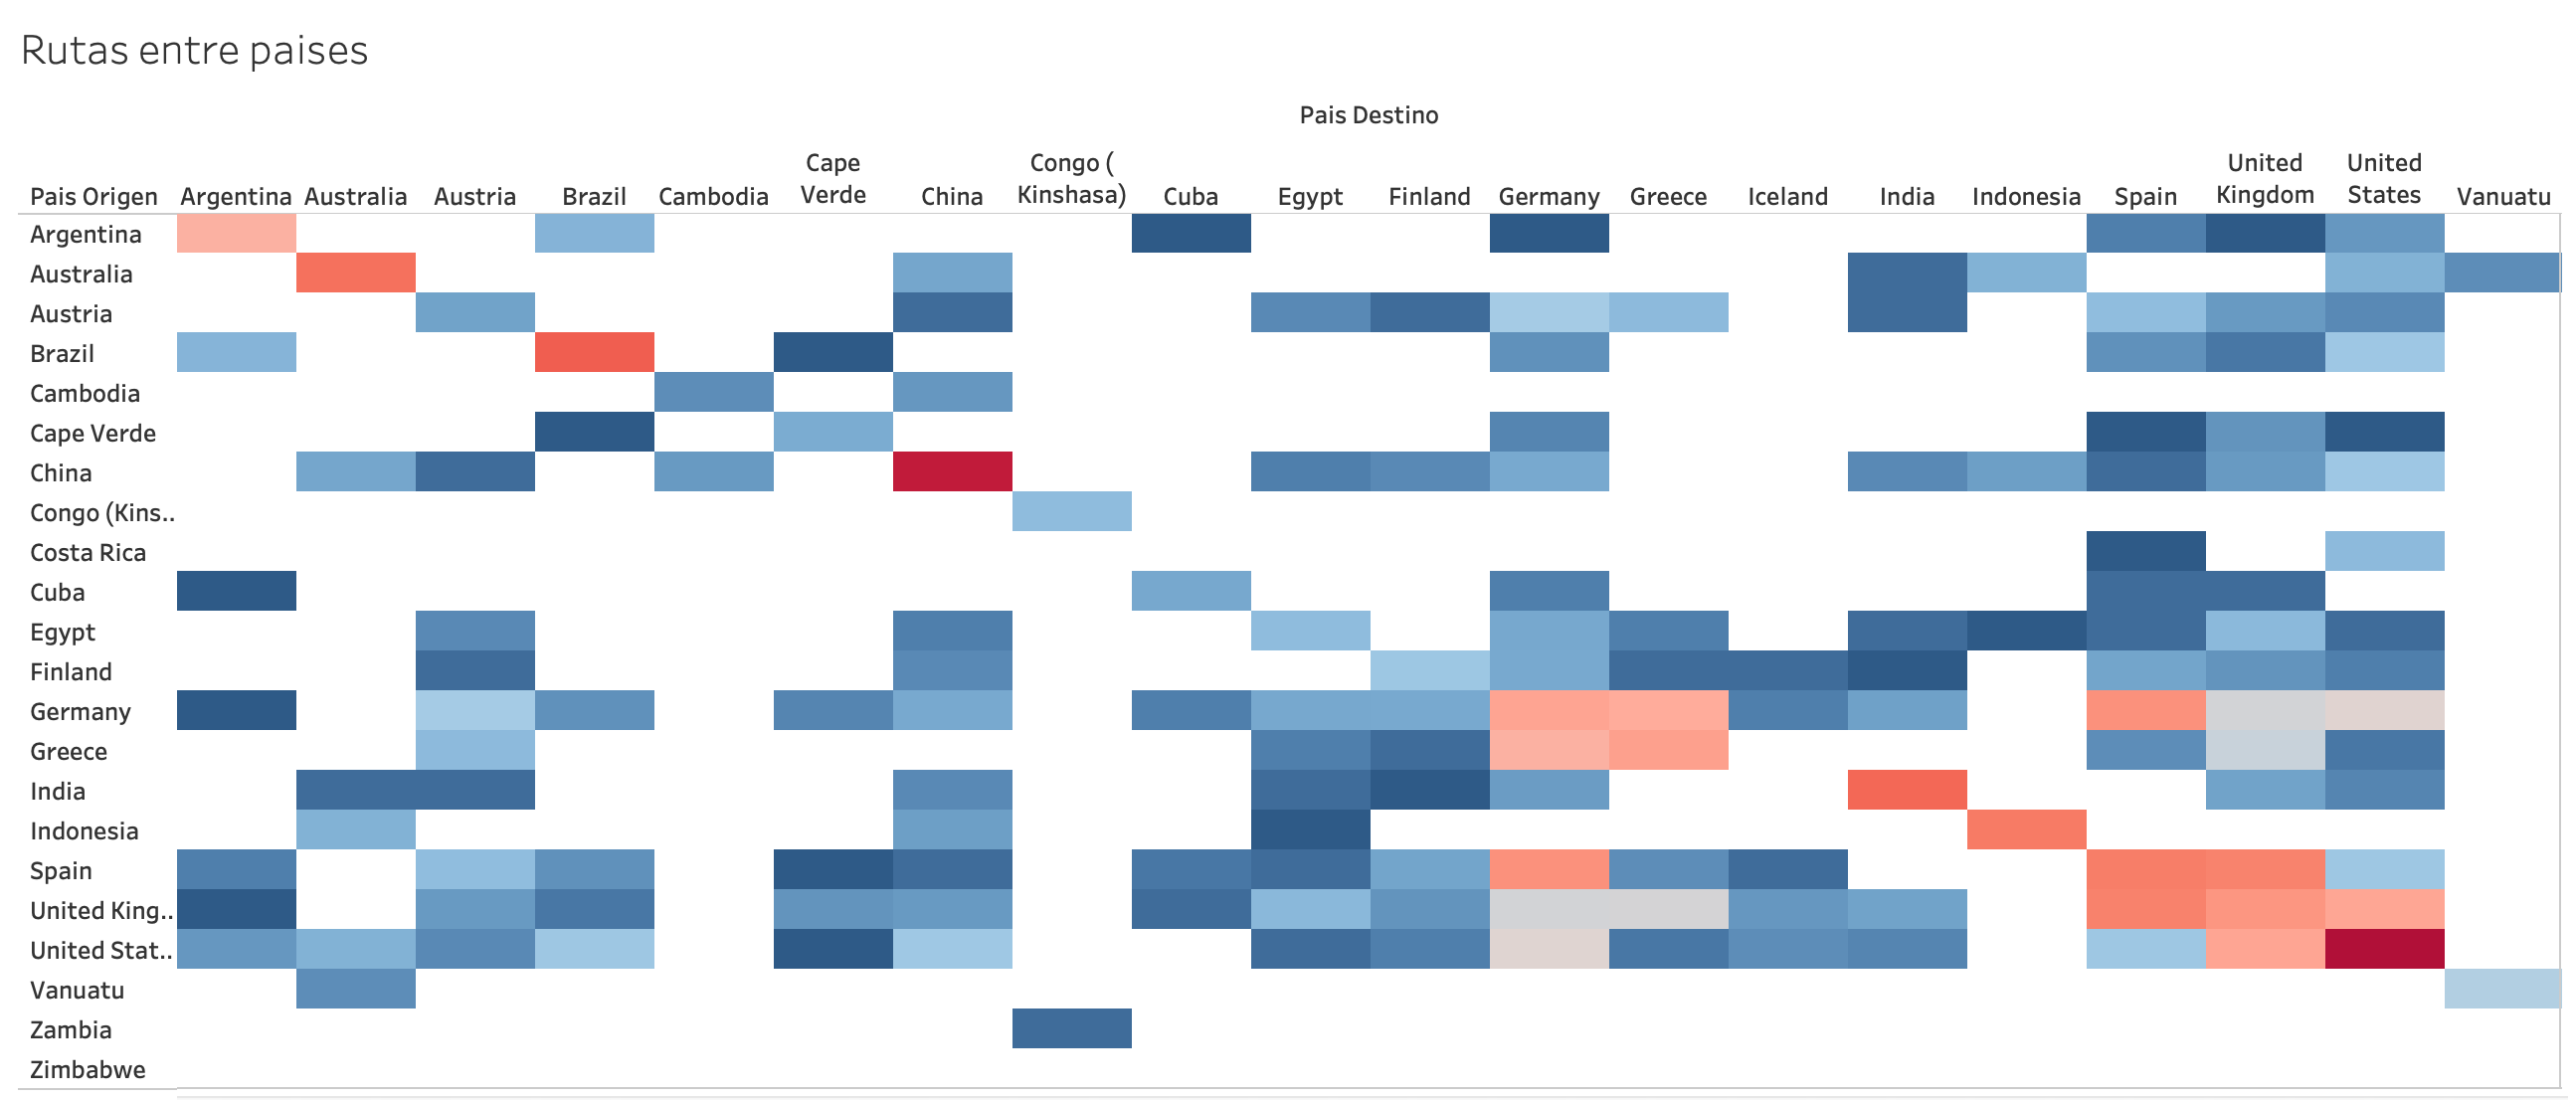
\includegraphics[width=\textwidth]{fotos/3.png}
\caption{Matriz de calor del número de rutas entre países. Se filtran algunos países para mostrar una visualización rápida.}
\label{fig:3}
\end{figure}

A partir de los campos existentes y del construido para el visual anterior, la creación de esta matriz es sencilla. Se usarán los campos \textit{Pais Destino} y \textit{Pais Origen} como columnas y filas, respectivamente (estos son los campos \textit{country} de la tabla usada para los aeropuertos de destino y origen, simplemente fueron renombrados). Se hace uso de la misma escala logarítmica que para la visualización anterior, lo que permitirá usar ambos visuales en conjunto en el \textit{dashboard}. Para ello se agrega el campo \textit{rutasLog} a color y se coge la misma paleta de colores, fijando esta vez el valor superior como el valor superior de la escala creada para el mapa de calor. De este modo, tenemos la misma interpretación visual que en el caso anterior: cuánto más oscuro sea el rojo, más rutas, y cuánto más oscuro sea el azul, menos rutas. En este caso, el uso de la escala logarítmica es crucial, ya que permite diferenciar países con una única ruta de conexión de países conectados por dos rutas; esto con la escala lineal sería imposible de diferenciar. \\

Para obtener información relevante, la descripción emergente de cada celda contendrá el pais de origen y destino (aunque ya venga en las filas y columnas, facilita la lectura en tablas grandes), junto con el número real de rutas:

\begin{lstlisting}[style=terminal]
Destino:	<Pais Destino>
Origen:	<Pais Origen>
Rutas:	<REC(routes)>
\end{lstlisting}

Aunque no se añadirán filtros aquí, el resultado para unos pocos países se muestra en la figura \ref{fig:3}. Esta matriz complementa muy bien al mapa de calor anterior; en la próxima sección se mostrará un ejemplo.




\section{\textit{Dashboard}}

A continuación, se describe el montaje del \textit{dashboard} usando los tres visuales construidos. El resultado se muestra en la figura \ref{fig:4}. \\

Para acompañar a las representaciones descirtas anteriormente, ahora si añadirán filtros. El mapa de rutas se agrega en la esquina inferior izquierda, junto con su leyenda y un filtro propio para el país de origen. Debido a la complejidad en el número de rutas, se configura para poder elegir un único país y ver sus rutas; agregar varios resultaría en una visualización que no aportaría ningún tipo de información. \\

El resto del \textit{dashboard} está dedicado al número de rutas de cada país y entre países. Como se comentó antes, se usa la misma escala para los dos, por lo que se tiene una leyenda única para ambos mapas. Se añaden dos filtros compartidos para ambos visuales: 
\begin{itemize}
\item Filtro por país de origen. Al seleccionar uno o varios países, estos se verán en el mapa de calor y se añadirán como filas a la matriz de calor. Como este filtro debe poder permitir seleccionar varios países, no se comparte con el filtro de país de origen del mapa de rutas. 
\item Filtro por número de rutas. Aquí se usa la escala lineal, ya que al tratarse de un filtro, lo numéricamente intuitivo es usar esta escala (recordemos que con la escala logarítmica simplemente ganamos interpretabilidad en los visual). Este filtro afecta también a ambos visuales, eliminando los valores que no cumplan con los criterios seleccionados.
\end{itemize}

Por último, debido a la cantidad de países, resulta necesario añadir un filtro adicional a la matriz de calor para seleccionar el o los países de destino a analizar. Los países seleccionados se añadirán entonces como columnas, pero sin tener esta vez ningún tipo de efecto sobre los el mapa de calor. Este filtro debe permitir también seleccionar varios países. \\

\begin{figure}[h]
\centering
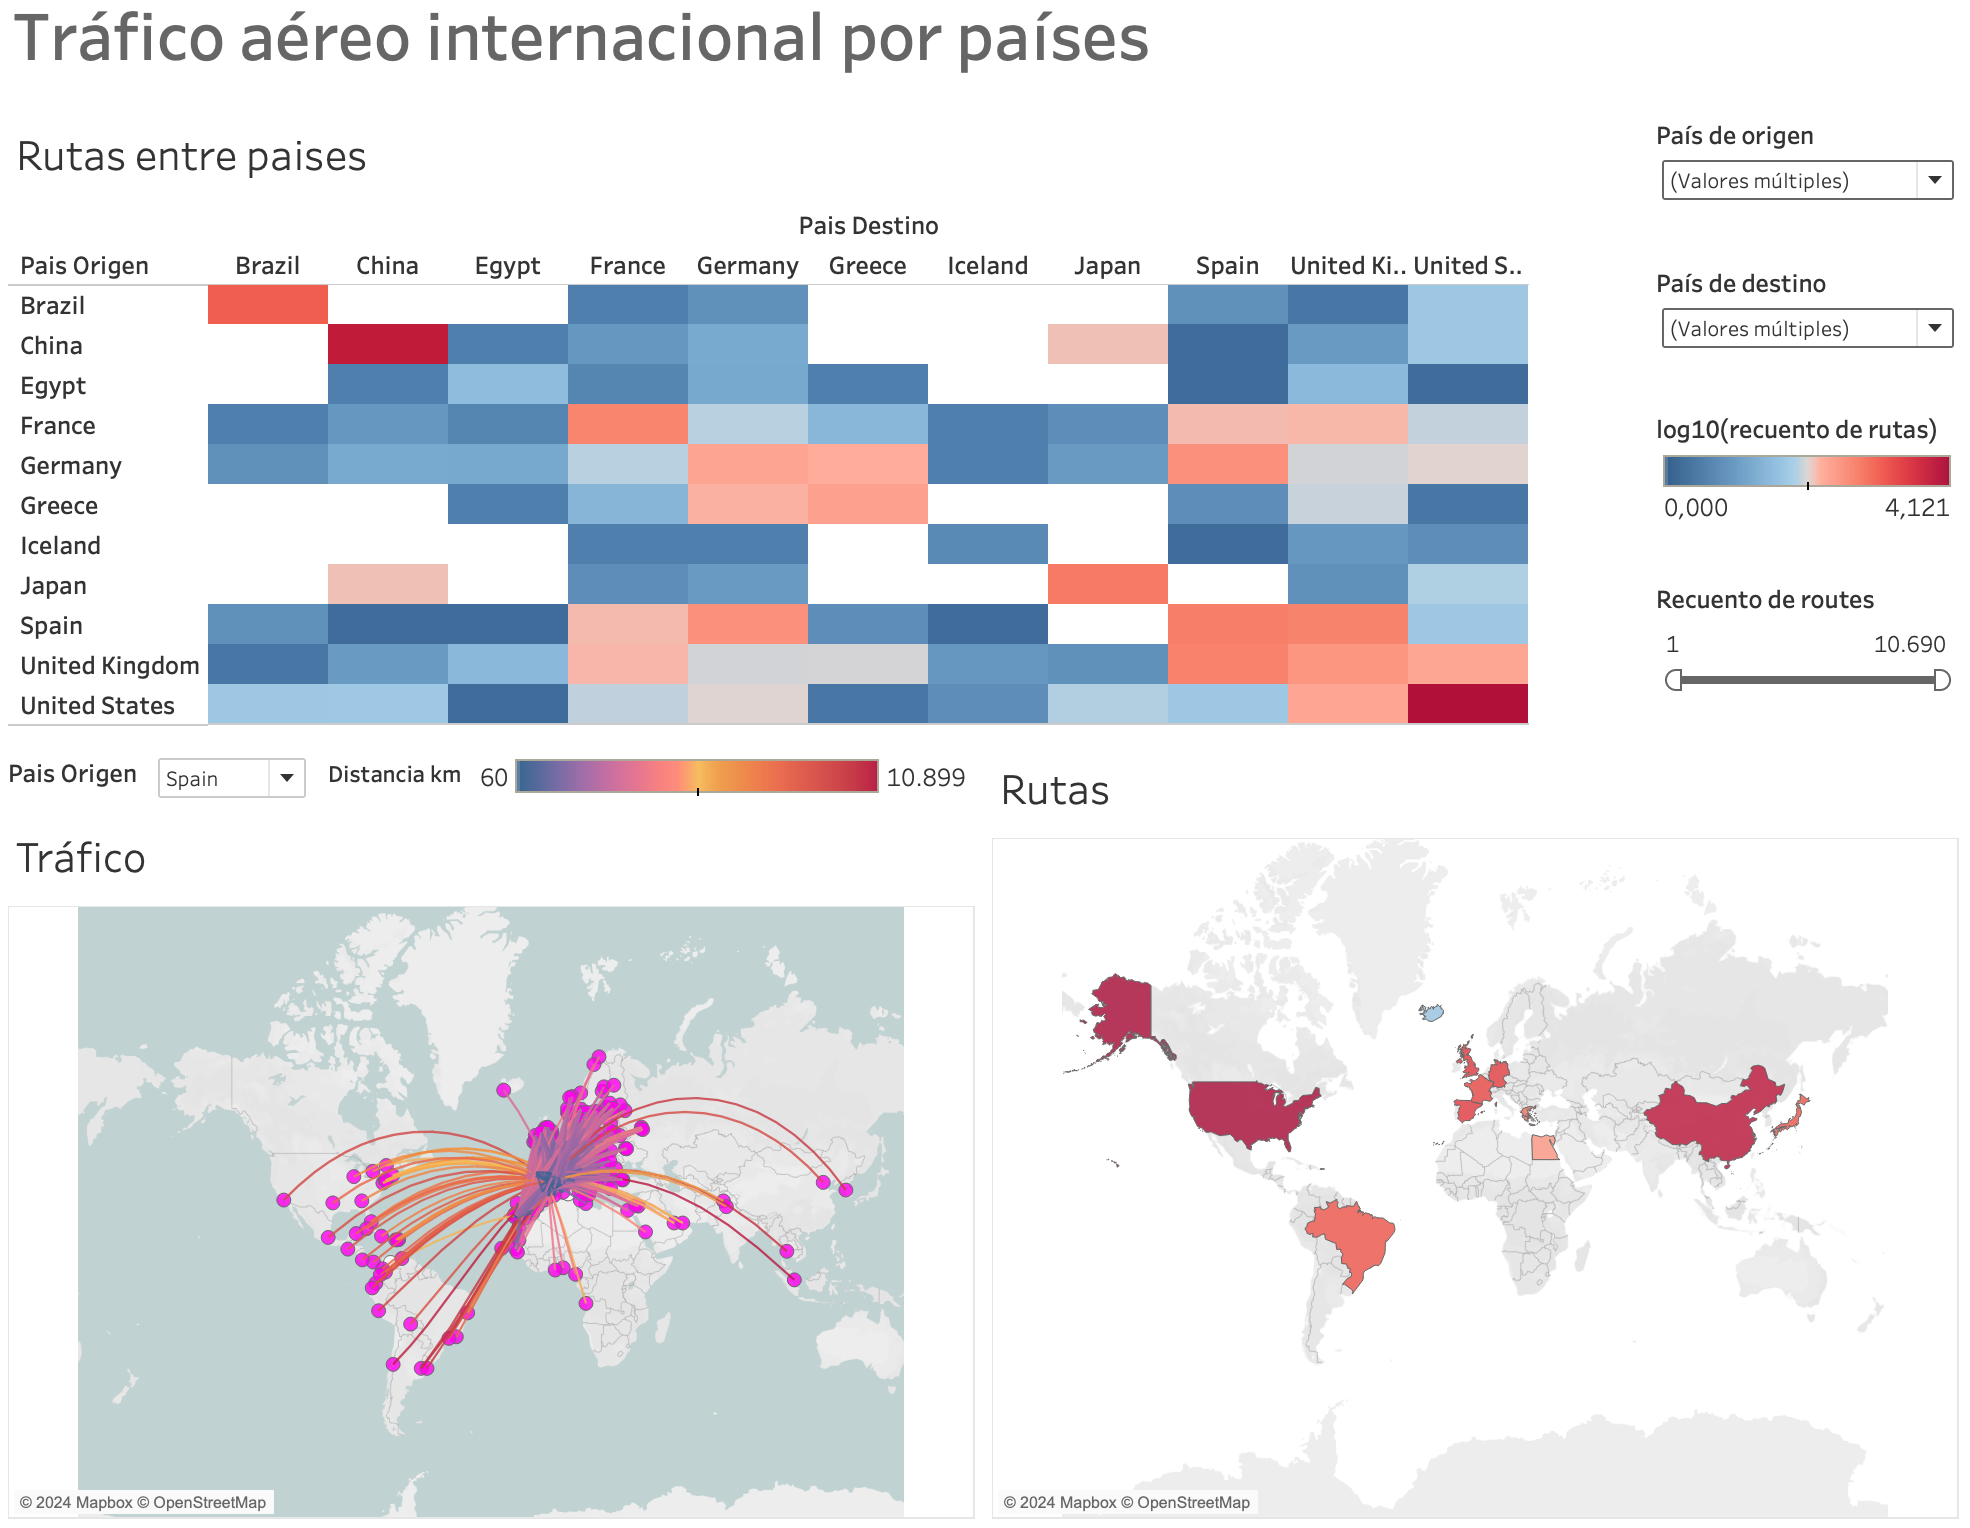
\includegraphics[width=\textwidth]{fotos/4.png}
\caption{\textit{Dashboard} del tráfico aéreo internacional.}
\label{fig:4}
\end{figure}

En la figura \ref{fig:4} se han tomado varios países como ejemplo para el visual. Para ver cómo se complementan el mapa y la matriz de calor, analicemos de forma rápida el top 4 países con mayores rutas globales: E.E.U.U., China, Reino Unido y España. A partir de la matriz de calor, sacaremos el número de rutas nacionales (es decir, que conectan a un país con él mismo), y a partir del mapa de calor obtendremos el número total de rutas de ese país. \\

Los dos primeros presentan un gran número de rutas nacionales: numéricamente, el 85\% de los rutas de China son nacionales, mientras que el este tipo de rutas suponen un 80\% del tráfico aéreo de E.E.U.U. En Reino Unido y España, esos porcentajes se reducen a un 11 y un 22\%, respectivamente. De hecho, Reino Unida presenta más de 1.5 veces más conexiones aéreas con España que nacionales. 
\end{document}
